\section{Experimentación}

Presentaremos en esta sección la experimentación, resultados y su discusión juntas para cada experimento. Primero daremos una breve descripción de la instancia experimental, seguido de lo que esperamos observar, es decir, nuestra hipótesis. A continuación mostraremos los resultados obtenidos y nuestro análisis respecto a por qué obtuvimos dichos resultados.

\subsection{Metodología en la generación de instancias}

Para la creación de instancias de prueba, para evitar sesgar los experimentos y por una cuestión de practicidad, decidimos utilizar instancias generadas aleatoriamente utilizando numpy. Todo el código de generación de datos, así como para correr los experimentos, y las instancias utilizadas para la experimentación, se encuentran en la carpeta experimentos; el archivo de ipython Experimentacion.ipynb contiene instrucciones explícitas sobre cómo generar instancias y correr los experimentos, y las carpetas de outputs tienen todas las salidas del programa aquí presentadas. Todas las visualizaciones y gráficos fueron creadas utilizando Tableau, y son reproducibles utilizando el archivo Workbook.twb. En términos de las distribuciones utilizadas, en cada uno de los experimentos explicaremos las particularidades de la elección de distribución, pero aquí presentamos una tabla mostrando la distribución utilizada para la generación de los parámetros de las sanguijuelas:

\begin{center}
\begin{tabular}{l | l | l | l | l | l | l}
Experimento & Instancia & \#Sanguijuelas & X & Y & Radio & Temperatura\\ \hline
$1$ & $1$ & $50$ & $\mathcal{U}(45, 55)$ & $\mathcal{U}(45, 55)$ & $|\mathcal{N}(0.5, 10)|$ & $\mathcal{E}(1/100)$\\ \hline
$1$ & $2$ & $50$ & $\mathcal{U}(0, 100)$ & $\mathcal{U}(0, 100)$ & $|\mathcal{N}(2, 100)|$ & $\mathcal{E}(1/100)$\\ \hline
$1$ & $3$ & $50$ & $\mathcal{U}(0, 100)$ & $\mathcal{U}(0, 100)$ & $|\mathcal{N}(0.1, 10)|$ & $\mathcal{E}(1/300)$\\ \hline
$2$ & $1$ & $50$ & $\mathcal{U}(0, 100)$ & $\mathcal{U}(0, 100)$ & $\mathcal{U}(0, 10)$ & $\mathcal{E}(1/300)$\\ \hline
$3$ & $1$ & $31$ & Explicado & Explicado & Explicado & $\mathcal{E}(1/300)$\\ \hline
\end{tabular}
\end{center}

Todas las instancias son de $100x100$ mts. La elección de los valores de $h$ fue una tarea complicada: la restricción de $h | a \wedge h | b$ restringe ampliamente el conjunto de valores (originalmente no nos dimos cuenta de esto, y las mediciones no tenían sentido). En sí, para tomar el $h$ agarramos una lista de los valores del $0.01$ al $100$, incrementados con diferencias de $0.01$, y nos fijamos cuales dividían a $100$ de la forma en que pide el enunciado. Terminamos viendo que

$$h \in \{0.01, 0.02, 0.04, 0.05, 0.08, 0.16, 0.2, 0.25, 0.4, 0.5, 0.8, 1.0, 1.25, 2.0, 2.5, 4.0, 5.0, 6.25, 10.0, 12.5, 50.0\}$$

Funcionaría bien para las instancias particulares que pensábamos utilizar. Descartamos el $h = 50$ por ser un valor demasiado grande, que resaltaría demasiado en las visualizaciones, y no aportaría demasiado por darnos una discretización demasiado pequeña, y comenzamos a probar cuál era la cota inferior de $h$ para correr los experimentos. Encontramos que utilizar valores de $h$ demasiado pequeños aumenta demasiado el costo computacional, como veremos más adelante. Es decir, intentar correr las instancias con un $h < 0.5$ terminaba por hacer que el equipo de pruebas no respondiera, obligándonos a reiniciar la computadora. Por lo tanto, nos decidimos a tomar

$$h \in \{0.5, 0.8, 1.0, 1.25, 2.0, 2.5, 4.0, 5.0, 6.25, 10.0, 12.5\}$$

Como conjunto de valores finales para la experimentación. En el caso particular del experimento 3 tomamos $h = 1$ por particularidades en el mecanismo de generación de instancias de test que comentaremos más adelante. Explicaremos la elección de las distribuciones de probabilidad en cada experimento particular.

Queremos destacar que hay que tener cuidado con la generación de instancias aleatorias: no necesariamente todas las instancias generadas por las distribuciones que mencionamos tienen las propiedades que buscamos en cada experimento, pudiendo tomar más de un intento para llegar a instancias que cumplan con las propiedades buscadas de cada instancia en particular. Dependiendo del experimento, tuvimos que intentar varias veces para lograr llegar a instancias que nos parecieran que cumplen con los criterios que enunciamos para correr el experimento, y el mismo fue un proceso de prueba y error, donde realmente no tenemos un criterio fijo para decir cuando una instancia cumple con las expectativas. Sí podemos afirmar que sobre las instancias que tomamos, las propiedades que enunciamos efectivamente se cumplieron como explicamos más adelante.

\subsection{Experimento 1: temperatura en función de la granularidad}

Para este experimento, nos planteamos como objetivo estudiar la relación entre la matriz de temperaturas final, la granularidad, y la distribución de las sanguijuelas. Desde el punto de vista algorítmico, notemos que la granularidad impacta en las sanguijuelas que terminan determinando la temperatura inicial de los puntos: si una sanguijuela es lo suficientemente chica y está ubicada de forma tal que su radio no llega a impactar en el punto de la discretización más cercano, no será considerada como parte de la matriz. Más aun, es importante advertir que las elecciones impuestas sobre el modelado generan condiciones extrañas: cuando dos sanguijuelas se superponen en un punto, se tomará el máximo de las temperaturas como la inicial para el punto. Es decir, existen instancias donde el aumento de granularidad (y por lo tanto la aparición de sanguijuelas de radio pequeño) efectivamente termina borrando sanguijuelas que antes existían, reemplazándolas por otras de mayor temperatura. Lo que buscamos remarcar con esto es que es difícil predecir el efecto que va a tener el cambio de granularidad sobre la matriz final de temperaturas cuando comienzan a haber más sanguijuelas, ya que la interacción de la discretización con las mismas se vuelve cada vez más complicada.

El primer experimento que ideamos consiste en crear una instancia donde todas las sanguijuelas estén muy cercanas al punto crítico, con radios lo suficientemente pequeños como para que el efecto de desaparición que mencionamos antes logre entrar en acción. Tras un largo proceso de prueba y error, determinamos que las distribuciones mencionadas anteriormente eran las que mejor modelaban la idea intuitiva que estábamos buscando probar. En particular, la elección de una distribución exponencial se debe a que buscamos que las sanguijuelas tengan valores relativamente pequeños para que borrarlas logre mostrarnos un cambio concreto en la temperatura del punto crítico. Para todos los casos del experimento 1 utilizamos el método de eliminación gaussiana para obtener las matrices de temperatura correspondientes. Sin embargo, el algoritmo de factorización LU debería devolver exactamente las mismas matrices de temperatura (ya que resuelven el mismo problema). Comprobamos de cualquier forma en nuestra experimentación que esto funcionaba así como forma de testear la correctitud del código fuera de las instancias provistas por la cátedra.

Intuitivamente esperábamos que la temperatura en el punto crítico fuera aumentando a medida que achicásemos el $h$: suponíamos que aumentar la granularidad forzosamente iba a resultar en que la mayor temperatura de las sanguijuelas cercanas al centro tomase relevancia en el punto crítico e iba a hacer que la temperatura del mismo subiese, mientras que tener una menor granularidad debía hacer que cada vez más sanguijuelas se perdieran en la discretización y forzaría a que las sanguijuelas mejor posicionadas para los nuevos valores de $h$ dominen la temperatura en el punto crítico. De las instancias que corrimos, creemos que el gráfico \ref{fig:exp11} es ampliamente representativo.

\begin{figure}[h]
    \centering
    \includegraphics[width=0.685\textwidth]{experimento 1-1}
    \caption{Variación de la temperatura en función de la granularidad para la primera instancia}
    \label{fig:exp11}
\end{figure}

\begin{figure}[h]
    \centering
    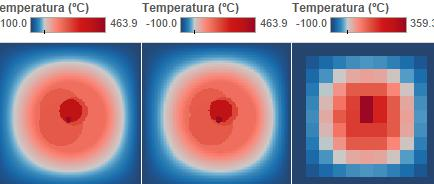
\includegraphics[width=0.685\textwidth]{Ejemplo Instancia 1}
    \caption{Mapa de calor para la instancia 1, tomando valores de $h = 0.5, 1, 10$}
    \label{fig:exp11-vis}
\end{figure}

Es fácil observar que la temperatura del punto critico se estabiliza a medida que aumenta la granularidad, y tiende a ser más bien caótico a medida que aumentamos el valor de h, es decir, disminuimos la granularidad. A diferencia de lo que esperábamos, la temperatura con mayor granularidad no es la mayor de las obtenidas, encontramos que la granularidad de la discretización es más bien un parámetro de regulación para la precisión de la solución: cuanta mayor granularidad, más difícil es que las sanguijuelas que aparezcan cambien sustancialmente la temperatura del punto crítico, ya que un $h$ más pequeño implica que los radios de las sanguijuelas que quedan por descubrir son lo suficientemente chicos como para afectar pocos puntos, y la ecuación de calor parece "balancear" las temperaturas hacia los valores más frecuentes. A modo de ayudar a la comprensión del experimento y la instancia contemplada, creamos una visualización del mapa de temperaturas generado por esta instancia particular, variando los valores de $h$ en la figura \ref{fig:exp11-vis}

Observemos que a medida que disminuimos la granularidad, el borde con temperatura $-100$ºC comienza a tomar cada vez más relevancia dentro de la discretización, y colabora aun más que antes a reducir los valores de temperatura.

Para la segunda instancia pensamos en crear sanguijuelas de un radio grande, en comparación con la primera instancia, alejadas del punto critico. En este caso esperábamos, en principio, que la temperatura se mantuviese constante a medida que aumentamos la granularidad, pues las sanguijuelas son lo suficientemente grandes para no desaparecer dentro de la discretización y más aun, esperamos una variación pequeña de temperatura en relación a la disminución de la granularidad. Observemos que en este caso cambiamos completamente la forma de generar las instancias de test, quitando restricciones en tanto a los valores de las sanguijuelas: el hecho de tomar distribución uniforme para las posiciones nos asegura la existencia de sanguijuelas en una variedad de puntos de la discretización, mientras que el radio normal nos da acceso a un panorama más variado en términos de los radios.

\begin{figure}[h]
    \centering
    \includegraphics[width=0.685\textwidth]{experimento 1-2}
    \caption{Variación de la temperatura en función de la granularidad para la segunda instancia}
    \label{fig:exp12}
\end{figure}

\begin{figure}[h]
    \centering
    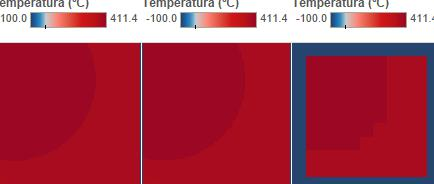
\includegraphics[width=0.685\textwidth]{Ejemplo Instancia 2}
    \caption{Mapa de calor para la instancia 2, tomando valores de $h = 0.5, 1, 10$}
    \label{fig:exp12-vis}
\end{figure}

La justificación de por qué la temperatura se estabiliza cercano a los $410$ºC es que hay una sanguijuela de aproximadamente $411$ºC y un radio muy grande, haciendo que abarque a muchos puntos de la discretización por más variación del h que haya. Con su radio, llega hasta el punto crítico y siempre le gana en temperatura a las sanguijuelas cercanas, ya que es la de mayor temperatura en esta instancia, y eso hace que le aumente la temperatura a los puntos de la discretización que no tienen sanguijuelas cercanas, como por ejemplo los puntos cercanos al centro del parabrisas pero que están del otro lado de la sanguijuela más caliente y no tienen ninguna sanguijuela a su alrededor. Al promediarse la temperatura en esos puntos, hace que la temperatura en el punto crítico sea cercana a los $410$ºC.

Observemos, en la figura \ref{fig:exp12}, que efectivamente la diferencia de temperatura entre el primer y el último h es baja, menor a $5$ºC, confirmando nuestra hipótesis sobre la variación de la temperatura a lo largo del aumento de granularidad. Una vez más encontramos que el algoritmo converge a una solución a partir de cierto $h$ y se mantiene estable, aunque la diferencia en este caso es que el $h$ viene antes que en la instancia 1. Una vez más, proveemos una visualización de la clase generada para la instancia 2 en el gráfico \ref{fig:exp12-vis}. Notemos que esta instancia es un muy buen ejemplo del segundo efecto de "desaparición" de sanguijuelas que mencionábamos antes: en este caso, en lugar de desaparecer por un cambio en el $h$, las sanguijuelas desaparecieron a causa de otra lo suficientemente alta en temperatura y radio.

Como tercera instancia, nos planteamos ver qué sucede con las sanguijuelas más pequeñas al estar alejadas del centro. Para esto, generamos instancias con las distribuciones mencionadas anteriormente, pero observemos que en este caso tomamos la temperatura como una variable exponencial de esperanza $300$, es decir, tomamos valores de temperatura mucho más altos. Nuestro análisis de los casos anteriores nos induce a pensar que las sanguijuelas suficientemente pequeñas no tendrán tanta relevancia en la temperatura del punto critico final. Esto es porque al afectar pocos puntos de la discretización, la ecuación de calor compensa esos valores al alejarse de la posición de las sanguijuelas. 

\begin{figure}[h]
    \centering
    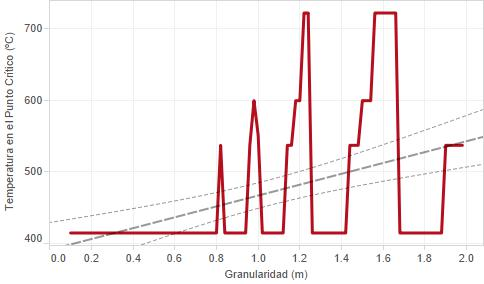
\includegraphics[width=0.685\textwidth]{experimento 1-3}
    \caption{Variación de la temperatura en función de la granularidad para la tercera instancia}
    \label{fig:exp13}
\end{figure}

\begin{figure}[h]
    \centering
    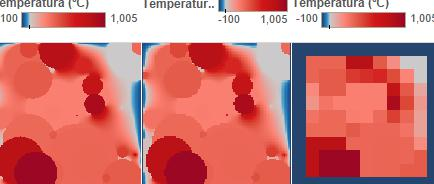
\includegraphics[width=0.685\textwidth]{Ejemplo Instancia 3}
    \caption{Mapa de calor para la instancia 3, tomando valores de $h = 0.5, 1, 10$}
    \label{fig:exp13-vis}
\end{figure}

En el gráfico \ref{fig:exp13} podemos observar que la temperatura solo varia, para una granularidad muy baja, en el orden de los $20$ºC. Sin embargo, a diferencia de los casos anteriores, encontramos que la temperatura se estabiliza a valores cada vez mas bajos al aumentar la granularidad, que efectivamente es lo que hipotetizamos que sucedería. Para profundizar la comprensión, podemos ver en el gráfico \ref{fig:exp13-vis} los mapas de calor correspondientes a la tercera instancia.

Es interesante cómo, a causa de los valores tan pequeños en el radio, el efecto de las sanguijuelas se ve disperso: por ejemplo, la sanguijuela de temperatura máxima es de $1000$ºC y sin embargo, la temperatura nunca supera los $270$ºC, ya que al estar tan separada del centro (aproximadamente localizada en el $(89, 29)$) y no tener un radio tan grande ($14.42$), no abarca muchos puntos de la discretización y la temperatura se va perdiendo a medida que nos vamos acercando al punto crítico.

Esto es una consecuencia directa de notar que a medida que aumenta la granularidad, la disipación de temperatura aumenta. Observando el mapa de calor mayor granularidad, parece que los altos valores de temperatura se limitan al área cubierta por las mismas, mientras que la temperatura desciende drásticamente al salir del radio. Se puede, sin embargo, observar áreas de calor entre dos sanguijuelas relativamente cercanas. Es decir, podemos concluir que el $h$ también funciona como un parámetro disipador de temperaturas, en el sentido que aumenta las distancias que debe cubrir una sanguijuela para lograr llegar al punto crítico por la forma que tiene la ecuación de calor.

\subsection{Experimento 2: relación entre tiempo de cómputo y calidad de la solución}

Para este experimento, buscábamos complementar los conocimientos adquiridos en el experimento anterior: sabíamos que cuanta mayor granularidad teníamos, más precisa es nuestra solución, y teníamos claro que tomar valores de $h$ muy pequeños no nos permitía solucionar los problemas por la excesiva carga computacional. Ahora lo que faltaba entender mejor es cuál es la relación entre el costo computacional y la granularidad. Para esto, utilizamos la tercera instancia que habíamos creado en el experimento anterior y medimos los tiempos de ejecución del algoritmo, la metodología utilizada fue correr el programa $5$ veces por cada valor de $h$, y tomar el promedio de los tiempos reportados. Para medir los tiempos de resolución, utilizamos la función gettimeof day, que permite medir con facilidad el lapso de tiempo entre dos momentos de la ejecución del programa; es importante destacar que todos los tiempos medidos representan exclusivamente el tiempo que tomó resolver la instancia del problema.

En el gráfico \ref{fig:exp21} podemos observar, en el primer casillero, la comparación entre los algoritmos, mientras que el segundo muestra la dimensión de la matriz del sistema a resolver (un punto $(h, d)$ en el gráfico se corresponde con una matriz final de $d \times ([\frac{a}{h}] + 1)$, tomaremos de aquí en adelante a $n$ como este $d$, ya que buscamos acotar superiormente la complejidad temporal). Observemos que las filas de la matriz del sistema crecen a la razón de $f(h) = ([\frac{a}{h}] + 1)([\frac{b}{h}] + 1)$, que es una función decreciente, con límite a $+\infty$ cuando $h$ tiende a $0$. Es importante destacar que este gran crecimiento de la matriz impacta muy fuertemente sobre el costo computacional, ya que ambos algoritmos son $O(n^3)$ a pesar de las mejoras que alcanzamos explotando la estructura de banda de la matriz.

Concretamente, tenemos que el costo de realizar eliminación gaussiana y resolver el sistema usando backward substitution es de $\frac{2n^3}{3} + \frac{3n^2}{2} + O(n)$ para sistemas que no precisan hacer pivoteo ~\cite{burden} (cabe destacar que esto no contempla las optimizaciones que realizamos para explotar la estructura de banda). Mientras tanto, realizar la factorización LU y resolver utilizando forward y backward substitution toma $\frac{2n^3}{3} + 2n^2 + O(n)$ ~\cite{LUComplexity}. Observemos que el costo de la factorización LU es mayor por un sumando de $\frac{n^2}{2}$, pero la explosión de complejidad que terminamos teniendo en las filas de la matriz hacen que este $n$ se dispare, generando la amplia diferencia que vemos en el gráfico \ref{fig:exp21}.

\begin{figure}[H]
    \centering
    \includegraphics[width=0.685\textwidth]{experimento 2-1}
    \caption{Comparación entre Eliminación Gaussiana y Factorización LU como métodos para resolver un sistema de ecuaciones con las características del trabajo práctico. El segundo gráfico se corresponde con la cantidad de filas de la matriz del sistema a resolver en función de $h$, para instancias de $100x100$ m. }
    \label{fig:exp21}
\end{figure}

Para investigar más en profundidad estos resultados y poder entender mejor la diferencia en performance de los algorítmos, basta tomar a la diferencia entre la complejidad de la resolución con LU y eliminación gaussiana, $\frac{n^2}{2}$, y evaluarla en la función $f$ que nos determina la cantidad de filas en función de $h$. Esto nos da: $g(h) = \frac{([\frac{a}{h}] + 1)^2 ([\frac{b}{h}] + 1)^2}{2}$ como la cantidad de operaciones extra que realiza LU en función de la granularidad de la discretización. Graficamos estos valores en la figura \ref{fig:exp21-cmp}. Observemos que la diferencia en crecimiento de complejidad teórica crece ampliamente con el decremento de $h$, llevando a que la diferencia real de ambas metodologías se muestre más claramente. Es muy importante tener en consideración que, dado que nuestros algoritmos sí explotan la estructura de banda, la primer curva toma valores mucho menores, pero sigue teniendo el mismo tipo de comportamiento en lineamientos generales y es por eso que incluimos el gráfico.

\begin{figure}[H]
    \centering
    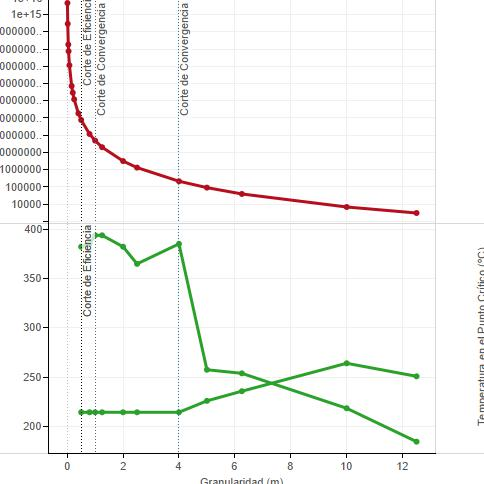
\includegraphics[width=0.8\textwidth]{Eficiencia de LU vs Gaussiana}
    \caption{Diferencia de complejidad temporal teórica entre los métodos y convergencia al punto crítico en función de H, respectivamente. La escala del primer gráfico es logarítmica, porque los valores se vuelven demasiado grandes muy repentinamente; cabe destacar que tomamos $a = b = 100$ para que la comparación tenga sentido. El corte de convergencia 1 está puesto en 4, el corte de convergencia 2 está puesto en 1, y el corte de eficiencia está puesto en 0.5. Las instancias graficadas en el segundo casillero son las 1 y 3 de las propuestas anteriormente.}
    \label{fig:exp21-cmp}
\end{figure}


En conclusión, encontramos que dependiendo de la instancia particular que tomemos podemos lograr converger con valores de $h$ tan grandes como $4$ (que inclusive es una buena aproximación en la instancia 1, donde la verdadera convergencia se encuentra en $h < 1$), pero que esta condición depende ampliamente de la distribución, los radios, y las temperaturas de las sanguijuelas. Además, confirmamos que siempre es mejor utilizar eliminación gaussiana en lugar de la factorización LU para resolver el problema de encontrar la matriz de temperaturas sin ninguna hipótesis adicional, y que este dato se vuelve por sobre todas las cosas relevante cuando estamos intentando resolver sistemas de mayor granularidad.

\subsection{Experimento 3: comparación entre algoritmos para eliminación de sanguijuelas}

En este experimento nos enfocamos en analizar las diferencias entre los algoritmos de eliminación de sanguijuelas, a los que llamaremos eliminación simple y eliminación con Sherman-Morrison. Basados en los tests de correctitud, podemos afirmar que ambos algoritmos tienen el mismo comportamiento cualitativo. Es decir, ambos devuelven la misma solución. Por esto, el enfoque de este experimento es el análisis temporal de los experimentos. 

Antes de establecer hipótesis alguna, vamos a hacer un breve análisis del comportamiento esperado de cada algoritmo. En primer lugar tenemos el algoritmo de eliminación simple. Este algoritmo se limita a, iterando sobre todas las sanguijuelas, eliminar una y recalcular la matriz de temperatura. Este comportamiento es independiente de los atributos de las sanguijuelas en si, sino que, a primera vista, es esperable que la complejidad solo dependa de la cantidad de sanguijuelas. Luego tenemos eliminación con Sherman-Morrison; en este caso, si se vuelve relevante el radio de las sanguijuelas: el algoritmo evita recalcular toda la factorización si la sanguijuela afecta solo un punto de la discretización.

Es por esto, que diseñamos el experimento de modo que se pueda apreciar la diferencia en el modo de cómputo. Este consiste en un tablero de $100 \times 100$ mts$^2$, en el cual fijaremos la cantidad de sanguijuelas y el tamaño de la discretización. Para medir la performance de cada algoritmo, generamos instancias con $31$ sanguijuelas incrementando el porcentaje de sanguijuelas unitarias que se encontraban en cada instancia con diferencias de aproximadamente $10\%$. Todas las instancias se caracterizan por tomar $h = 1$, y disponer de las sanguijuelas en forma de grilla, es decir, ocupando las posiciones en orden desde la esquina inferior derecha por filas, hasta lograr cubrir las posiciones necesarias. Además, posicionamos una sanguijuela de $1000$ºC en el punto crítico, para asegurarnos que los algoritmos corran al tener la misma por encima de $235$ºC. La forma de generar sanguijuelas unitarias es, entonces, a través de tomar radios menores a $0.8$ y mayores a $0.2$, mientras que en el caso dual podemos tomar sanguijuelas de radio mayor a $1.1$ y menor a $1.4$. Observemos que el incremento podemos determinarlo como "aproximadamente" de $10\%$ debido a que las sanguijuelas "unitarias" que se encuentren en el límite con las sanguijuelas no unitarias van a tener su posición influenciada por más de 1 sanguijuela, haciendo que no pueda aplicarse Sherman Morrison. De cualquier forma, esta limitación no generó ninguna complicación, ya que la distorsión introducida en el porcentaje es lo suficientemente bajo como para que los resultados no varíen demasiado. En la figura \ref{fig:exp31-vis} mostramos un ejemplo de la distribución del calor luego de correr el algoritmo (que, como debería, borró la sanguijuela en el medio de la discretización).

\begin{figure}[H]
    \centering
    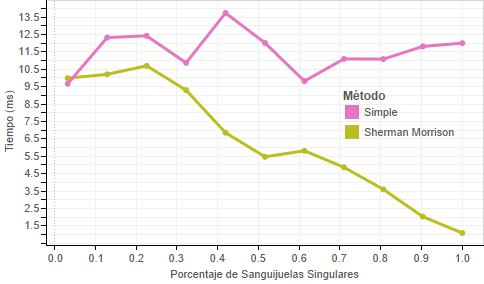
\includegraphics[width=0.685\textwidth]{experimento 3-1}
    \caption{Comparación entre SM y el método simple}
    \label{fig:exp31}
\end{figure}

\begin{figure}[H]
    \centering
    
\includegraphics[width=0.30\textwidth]{Ejemplo SM}
    \caption{Comparación entre SM y el método simple}
    \label{fig:exp31-vis}
\end{figure}

Si miramos los tiempos de ejecución para Sherman-Morrison en la figura \ref{fig:exp31}, podemos observar claramente que a medida que aumenta el porcentaje de sanguijuelas unitarias, el tiempo de computo disminuye. Esto se debe a que cada vez que debe analizar una sanguijuela unitaria puede aprovechar los resultados ya calculados: en lugar de recalcular la matriz entera e incurrir en el costo del algoritmo de eliminación gaussiana de complejidad $O(n^3)$, podemos aprovechar la factorización LU ya calculada y tomar un costo de $O(n^2)$. Por su parte, el algoritmo de eliminación simple mantiene un rango bajo de variación en las mediciones. Esto sucede porque independientemente del rango de las sanguijuelas, siempre debe recalcular el total de los datos al eliminar una, y eso incurre en un costo computacional alto.

Si comparamos la primer medición, donde todas las sanguijuelas afectan mas de un punto de la discretización, podemos notar que eliminación con Sherman-Morrison tiene un tiempo de computo ligeramente superior. Esto se debe a que en estos casos, Sherman-Morrison simplemente corre eliminación gaussiana para evitar incurrir en el costo de calcular la factorización LU de la matriz y desaprovechar recursos. Sin embargo, siguiendo la evolución del gráfico, vemos como esto queda claramente compensado a medida que van apareciendo sanguijuelas unitarias. Por lo tanto, concluimos que solo es viable usar eliminación simple cuando no hay ninguna posibilidad de encontrar sanguijuelas unitarias, o cuando sólo hay una sanguijuela unitaria; ya que en estos casos el costo de computar la factorización LU no será amortizado a la larga.